\chapter{Evaluation and results}
\label{chap:eval}

%todo outline
Short outline as usual.

%todo rework

\section{Datasets}
\label{sec:datasets}

\begin{itemize}
  \item Tsukuba Stereo Dataset (used Tsukuba Map as reference)
  \item Stereo videos with ground truth disparities from cambridge\footnote{\url{http://www.cl.cam.ac.uk/research/rainbow/projects/dcbgrid/datasets/}}
  \item SVDDD - a high-resolution Stereoscopic Video Dataset with precise Depth and Disparity information
\end{itemize}

%todo intro

\subsection*{Ground-truth data}

In general there exist two ways to gain ground-truth information of pixels:
\begin{itemize}
  \item in the real-world sense the area,
  \item in computer-animated scenes let the renderer calculate the disparity.
\end{itemize}

\noindent The former can be achieved via area scanner for instance a radar.
This approach is of course more error-prone than the latter one.
%todo find more examples
It can lack of accuracy due to false measurements.
The latter one provides real ground-truth information.

%todo explain errorbars
Provide real-world ground truth disparity maps \citep{kondermann2015stereo}.

\subsubsection*{Availability}

%todo explain
The aim of such datasets is to provide data which we can rely on to evaluate the performance of computer vision algorithms, such as disparity algorithms in this thesis.
 Without having such datasets it would be crucial to rate the overall quality of for instance stereo matching algorithms.

We use the datasets for stereo correspondences from Middlebury, cf.  \citep{scharstein2014high}. They provide us with three examples. Each of those examples include an image from each camera (left, right) and the resulting ground-truth disparity map.

We also use the small images from \citep{martull2012realistic}.

Famous Tsukuba ground-truth dataset:

\begin{itemize}
  \item 64 levels of disparity, so grayscale image
  \item generated scenes with Autodesk Maya 2012
\end{itemize}

\citep{martull2012realistic}

Ground truth data? How to provide such data?


\subsubsection{Tsukuba stereo dataset}

This dataset can be seen as the origin of stereoscopic datasets.
The first dataset ever released for working with stereoscopic images.
\citep{martull2012realistic}.

%todo intro

\subsubsection{Middlebury stereo dataset}

\citep{scharstein2014high}.

%todo intro

\subsubsection{Cambridge stereo dataset}

%todo intro
The Cambridge stereo dataset consists of five different rendered scenes in $400x300$ resolution with each about 100 frames \citep{richardt2010real}.
The dataset scales the disparity for each scene from $0$ to $64$.

\subsubsection{SVDDD - a high-resolution Stereoscopic Video Dataset with precise Depth and Disparity information}

The Lehrstuhl f{\"u}r Praktische Informatik IV\footnote{\url{http://ls.fmi.uni-mannheim.de/de/pi4/}} has created a novel dataset on its own containing depth information for stereoscopic videos.
Before the evaluation it was clear that this dataset is going to be evaluated as well.
The difference is that this dataset was not analyzed before.
Thus it is possible that the chosen algorithms work not properly on this dataset.
If this case occurs there exist two possibilities why this happens:

\begin{itemize}
  \item On the one hand, the disparity information are not properly calculated, or
  \item on the other hand, those algorithms have some troubles with the constructed scene.
\end{itemize}

\noindent Focusing on the latter one, the scenes were created with Blender and utilizes the XXX (insert me pls) open-source scenes.
A second camera was added to the scene for obtaining depth information.
The parameter for each scene can be extracted from the paper.
The most important points which can lead to a discrepancy between the computed disparity maps and the ground-truth data are the following:

\begin{itemize}
  \item rays of light were removed only in the ground-truth-data,
  \item motion and object blur was reduced only in the ground-truth data,
  \item fain-grained textures were reduced only in the ground-truth data.
\end{itemize}

%todo go into more concrete

\section{Quality metrics}

To evaluate the quality of computed disparity maps we need at first to what we compare the computed disparity maps to and secondly how to compare them. In the section \ref{chap:datasets} the availability of such datasets were discussed.

Insert table here.

\begin{table}[h!]
\centering
\begin{tabular}{l|l}
\textbf{Tag} & \textbf{Description} \\ \hline
$\sigma_{10}$ & Guassian noise calculator. \\ \hline
 &  \\ \hline
 &  \\
\end{tabular}
\caption{Overview on used metrics in results}
\label{tab:metrics}
\end{table}

\noindent Typical quality measure instruments for comparing disparity maps against their ground-truth reference data are  \citep{cyganek2011introduction}:

\begin{itemize}
  \item Percentage of bad matching pixels
  \item Root-mean-square error
  \item Parameter-free measures
\end{itemize}

In addition the following are also considered:

\begin{itemize}
  \item Mean absolute error in pixels
  \item Error quantiles
  \item Precision and accuracy
\end{itemize}

\subsection*{Percentage of bad matching pixels}

\begin{equation}
  \operatorname{PBMP}=\frac{1}{n} \sum_{x,y=0}^{}(|d_a(x,y) - d_e(x,y)| > \delta_t)
\end{equation}

\noindent Percentage of bad matching pixels for given threshold.

\subsection*{Root-mean-squared error}

The mean squared error (MSE) as well as the root mean squared error (RMSE) are both the most popular metrics in image and video processing.
The MSE is as the name implies the mean of the squared differences between the intensities of pixels in two pictures at the same position.
In conclusion the average difference per pixel is then the root of the squared error.

\begin{equation}
  \operatorname{RMS-Error}=\sqrt{\frac{1}{n} \sum_{x,y=0}^{}(d_a(x,y) - d_e(x,y))^2}
\end{equation}

\noindent It represents the sample standard deviation of the differences between predicted values and observed values.
Here $d_a(x,y)$ is the actual disparity value for given $x$ and $y$.
$d_e(x,y)$ is our expected disparity value from our ground-truth data.
Hence the RMSE is the difference between values on average.

\subsection*{Energy efficiency}

\begin{equation}
  EE_{alg} = \frac{clean\ pixels}{runtime\ in\ seconds}
\end{equation}

\noindent where $clean\ pixels$ are defined as bad pixels in percent of non-occluded pixels and $runtime\ in\ seconds$ the runtime for this particular frame. $EE_{alg}$ is then calculated in the mean of all frames of a given sequence over all examined sequences and all datasets.

\section{Measurement}

\begin{itemize}
	\item First took normal depth map images. But not that good, only values from 0-255.
	\item Actual evaluation process consists of comparison of real calculated values of depth map by results of algorithms.
	\item How does the eval actual look like?
\end{itemize} \citep{benoit2008quality}, \citep{scharstein2002taxonomy}.

\subsection*{Parameter tuning}

Our results.

\subsection*{Against reference dataset}

It is also important to have some kind of reference dataset with which the evaluation engine can be calibrated with.
Of course the settings (i.e. parameters of an algorithm) is dependent on the input material (size, noise) and on the scene (e.g. textured vs textureless).
So it is possible to have good parameters for one scene and not for another.
However, in order to evaluate those algorithms the Tsubuka stereo dataset was chosen as reference dataset to see how the eval engine actually works with the same parameters on the same images.

\section{Results}

The results are visualized with the HSV color model.

\begin{figure}[h!]
  \centering
  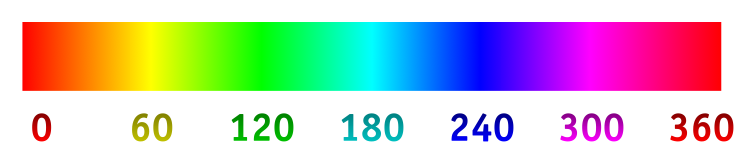
\includegraphics[width=0.8\textwidth]{src/images/hue-scale.png}
  \caption{Scale of hue of the HSV color model.}
  \label{fig:hue-scale}
\end{figure}

%todo results

\subsection*{Applying disparity algorithms on videos}

As said in the implementation chapter \ref{chap:impl} applying disparity algorithms on videos is trivial and straightforward.
None the less different anomalies can be further investigated while analyzing videos:

\begin{itemize}
  \item outliers in the form of a single frames which differs too much from the others,
  \item impact of noise,
  \item smooth the unknown disparity in frames (next subsection).
\end{itemize}

\noindent As you can see in the following result matrices the quality metrics regarding the salient regions are a bit esoteric. Of course there exist techniques to estimate salient regions in static images and also in videos. In videos moving objects can be detected as salient, referring to motion saliency\citep{opencv_library, wang2014fast}. None the less those bitmasks are a bit more esoteric in the sense of there is room for interpretation.

\begin{landscape}
  \begin{table}[h!]
  \centering
  \begin{tabular}{cll|rrrrr}
    \hline
    \textbf{Rank} & \textbf{Method} & \textbf{Sequence} & \textbf{RMS-All} & \textbf{RMS-Noc} & \textbf{RMS-Sal} & \textbf{RMS-Tex} & \textbf{RMS-DD} \\ \hline \hline
    1 & StereoSGBM & SVDDD 02\_rabbit & 4.35\% & \cellcolor{green!60}5.43\% & 1.0 px & 1.1 px & 300ms \\
    2 & StereoBM & SVDDD 02\_rabbit & 4.35\% & 5.43\% & 1.0 px & \cellcolor{red!60}1.1 px & 300ms \\ \hline
  \end{tabular}
  \caption{Result matrix of RMS for videos}
  \label{tab:result-videos-rms}
  \end{table}
\end{landscape}

\begin{landscape}
  \begin{table}[h!]
  \centering
  \begin{tabular}{cll|rrrrr}
    \hline
    \textbf{Rank} & \textbf{Method} & \textbf{Sequence} & \textbf{Out-All} & \textbf{Out-Noc} & \textbf{Out-Sal} & \textbf{Out-Tex} & \textbf{Out-DD} \\ \hline \hline
    1 & StereoSGBM & SVDDD 02\_rabbit & 4.35\% & \cellcolor{green!60}5.43\% & 1.0 px & 1.1 px & 300ms \\
    1 & StereoSGBM & SVDDD 02\_rabbit & 4.35\% & \cellcolor{green!60}5.43\% & 1.0 px & 1.1 px & 300ms \\
    1 & StereoSGBM & SVDDD 02\_rabbit & 4.35\% & \cellcolor{green!60}5.43\% & 1.0 px & 1.1 px & 300ms \\
    1 & StereoSGBM & SVDDD 02\_rabbit & 4.35\% & \cellcolor{green!60}5.43\% & 1.0 px & 1.1 px & 300ms \\
    1 & StereoSGBM & SVDDD 02\_rabbit & 4.35\% & \cellcolor{green!60}5.43\% & 1.0 px & 1.1 px & 300ms \\
    1 & StereoSGBM & SVDDD 02\_rabbit & 4.35\% & \cellcolor{green!60}5.43\% & 1.0 px & 1.1 px & 300ms \\
    1 & StereoSGBM & SVDDD 02\_rabbit & 4.35\% & \cellcolor{green!60}5.43\% & 1.0 px & 1.1 px & 300ms \\
    1 & StereoSGBM & SVDDD 02\_rabbit & 4.35\% & \cellcolor{green!60}5.43\% & 1.0 px & 1.1 px & 300ms \\
    1 & StereoSGBM & SVDDD 02\_rabbit & 4.35\% & \cellcolor{green!60}5.43\% & 1.0 px & 1.1 px & 300ms \\
    1 & StereoSGBM & SVDDD 02\_rabbit & 4.35\% & \cellcolor{green!60}5.43\% & 1.0 px & 1.1 px & 300ms \\
    1 & StereoSGBM & SVDDD 02\_rabbit & 4.35\% & \cellcolor{green!60}5.43\% & 1.0 px & 1.1 px & 300ms \\
    1 & StereoSGBM & SVDDD 02\_rabbit & 4.35\% & \cellcolor{green!60}5.43\% & 1.0 px & 1.1 px & 300ms \\
    1 & StereoSGBM & SVDDD 02\_rabbit & 4.35\% & \cellcolor{green!60}5.43\% & 1.0 px & 1.1 px & 300ms \\
    1 & StereoSGBM & SVDDD 02\_rabbit & 4.35\% & \cellcolor{green!60}5.43\% & 1.0 px & 1.1 px & 300ms \\
    1 & StereoSGBM & SVDDD 02\_rabbit & 4.35\% & \cellcolor{green!60}5.43\% & 1.0 px & 1.1 px & 300ms \\
    1 & StereoSGBM & SVDDD 02\_rabbit & 4.35\% & \cellcolor{green!60}5.43\% & 1.0 px & 1.1 px & 300ms \\
    1 & StereoSGBM & SVDDD 02\_rabbit & 4.35\% & \cellcolor{green!60}5.43\% & 1.0 px & 1.1 px & 300ms \\
    1 & StereoSGBM & SVDDD 02\_rabbit & 4.35\% & \cellcolor{green!60}5.43\% & 1.0 px & 1.1 px & 300ms \\
    1 & StereoSGBM & SVDDD 02\_rabbit & 4.35\% & \cellcolor{green!60}5.43\% & 1.0 px & 1.1 px & 300ms \\
    1 & StereoSGBM & SVDDD 02\_rabbit & 4.35\% & \cellcolor{green!60}5.43\% & 1.0 px & 1.1 px & 300ms \\
    1 & StereoSGBM & SVDDD 02\_rabbit & 4.35\% & \cellcolor{green!60}5.43\% & 1.0 px & 1.1 px & 300ms \\
    2 & StereoBM & SVDDD 02\_rabbit & 4.35\% & 5.43\% & 1.0 px & \cellcolor{red!60}1.1 px & 300ms \\ \hline
  \end{tabular}
  \caption{Result matrix of outliers for videos}
  \label{tab:result-videos-out}
  \end{table}
\end{landscape}



\begin{figure}[h!]
\centering
\begin{tabular}{cc}

\subfloat[Left image]{\includegraphics[width=0.47\textwidth]{src/images/svddd-03-left.png}} &
\subfloat[Right image]{\includegraphics[width=0.47\textwidth]{src/images/svddd-03-right.png}} \\

\subfloat[Ground-truth disparity]{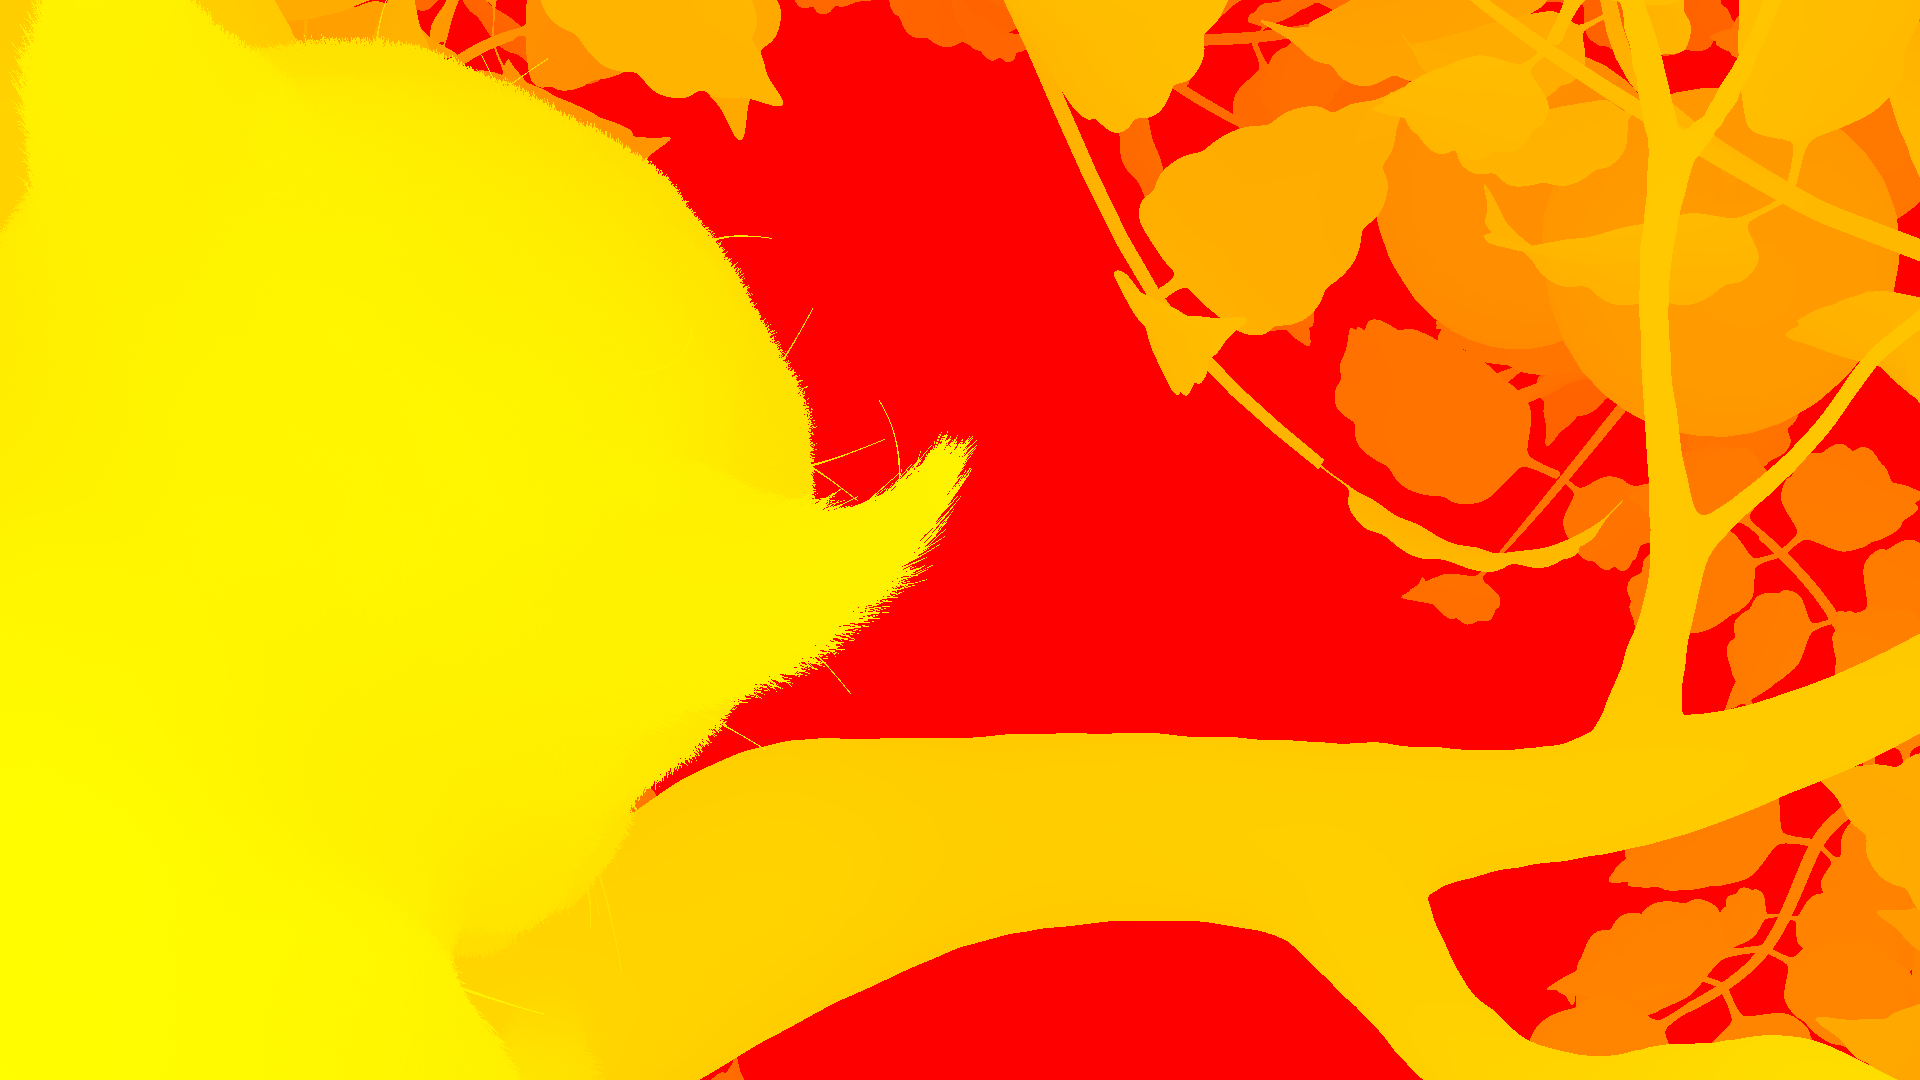
\includegraphics[width=0.47\textwidth]{src/images/svddd-03-heatmap-groundtruth.png}} &
\subfloat[SGBM output]{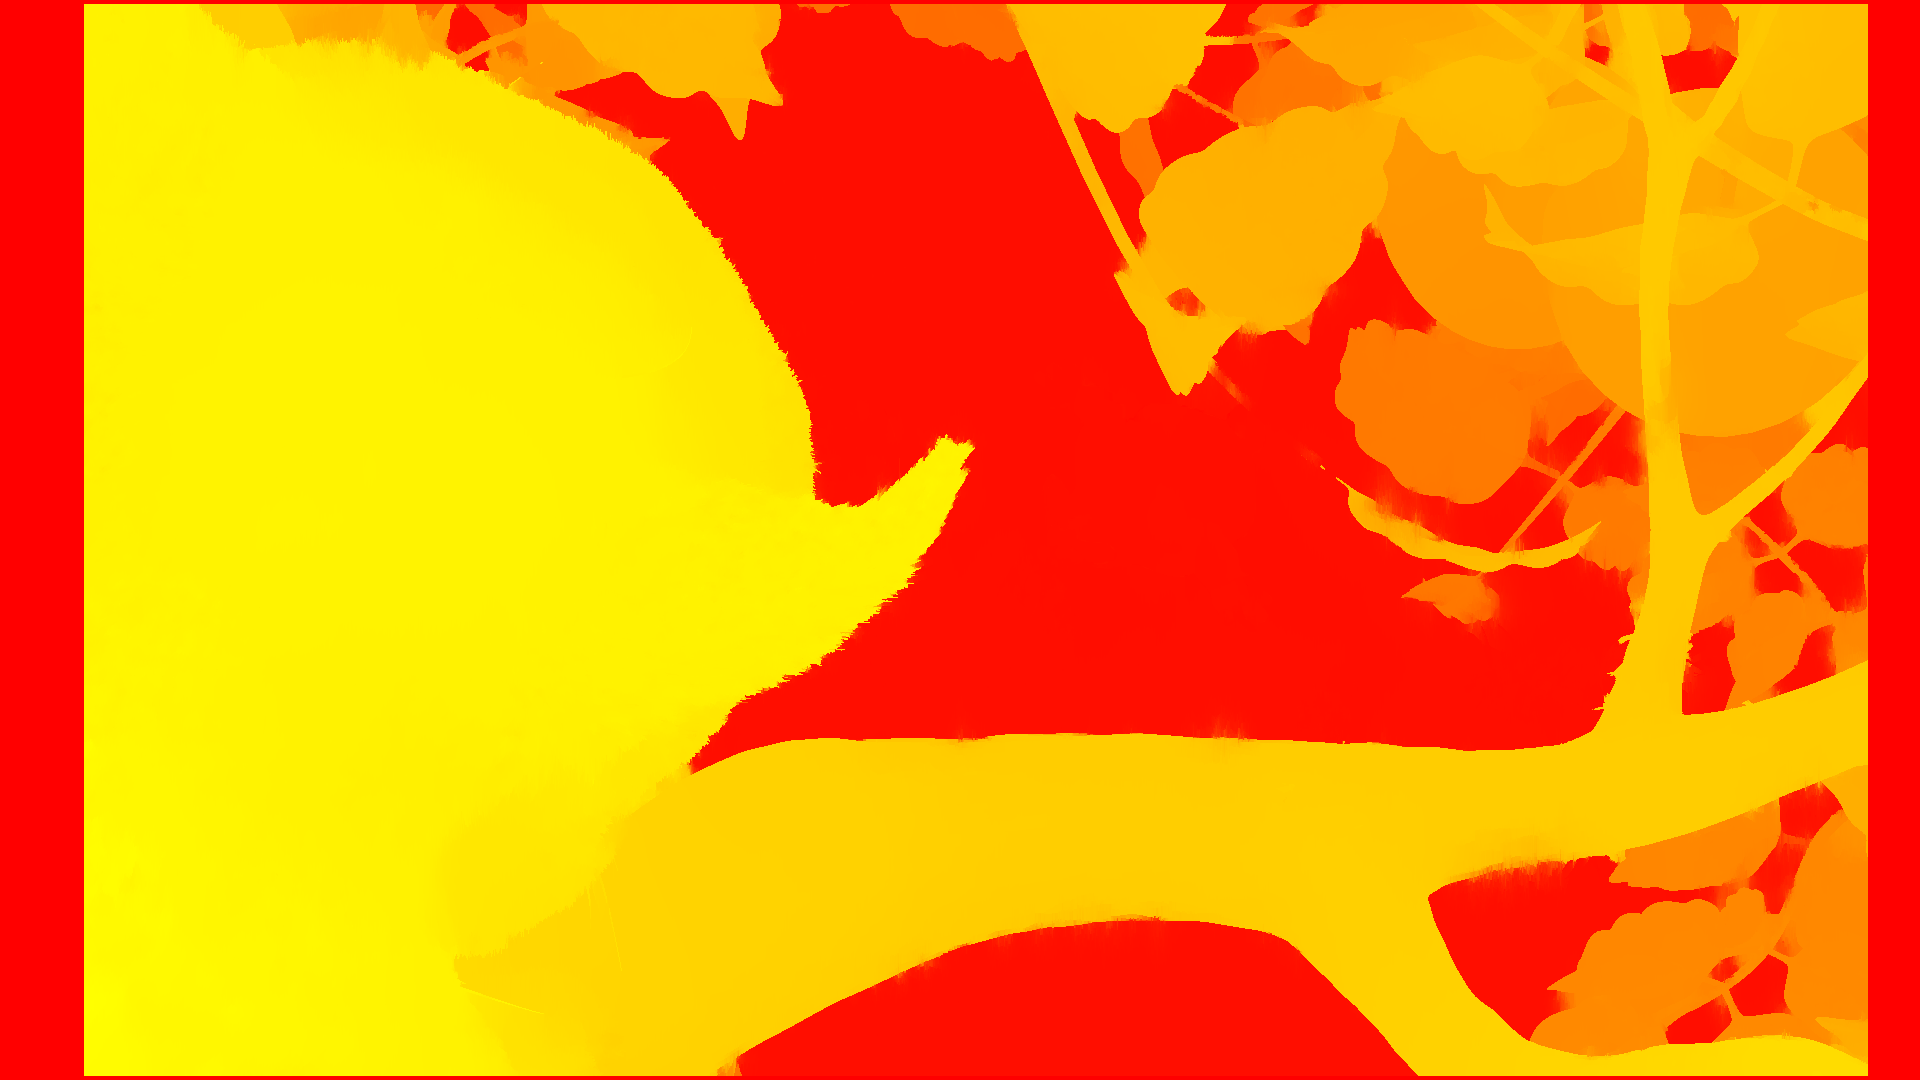
\includegraphics[width=0.47\textwidth]{src/images/svddd-03-heatmap-sgbm.png}} \\

\subfloat[MRF ICM output]{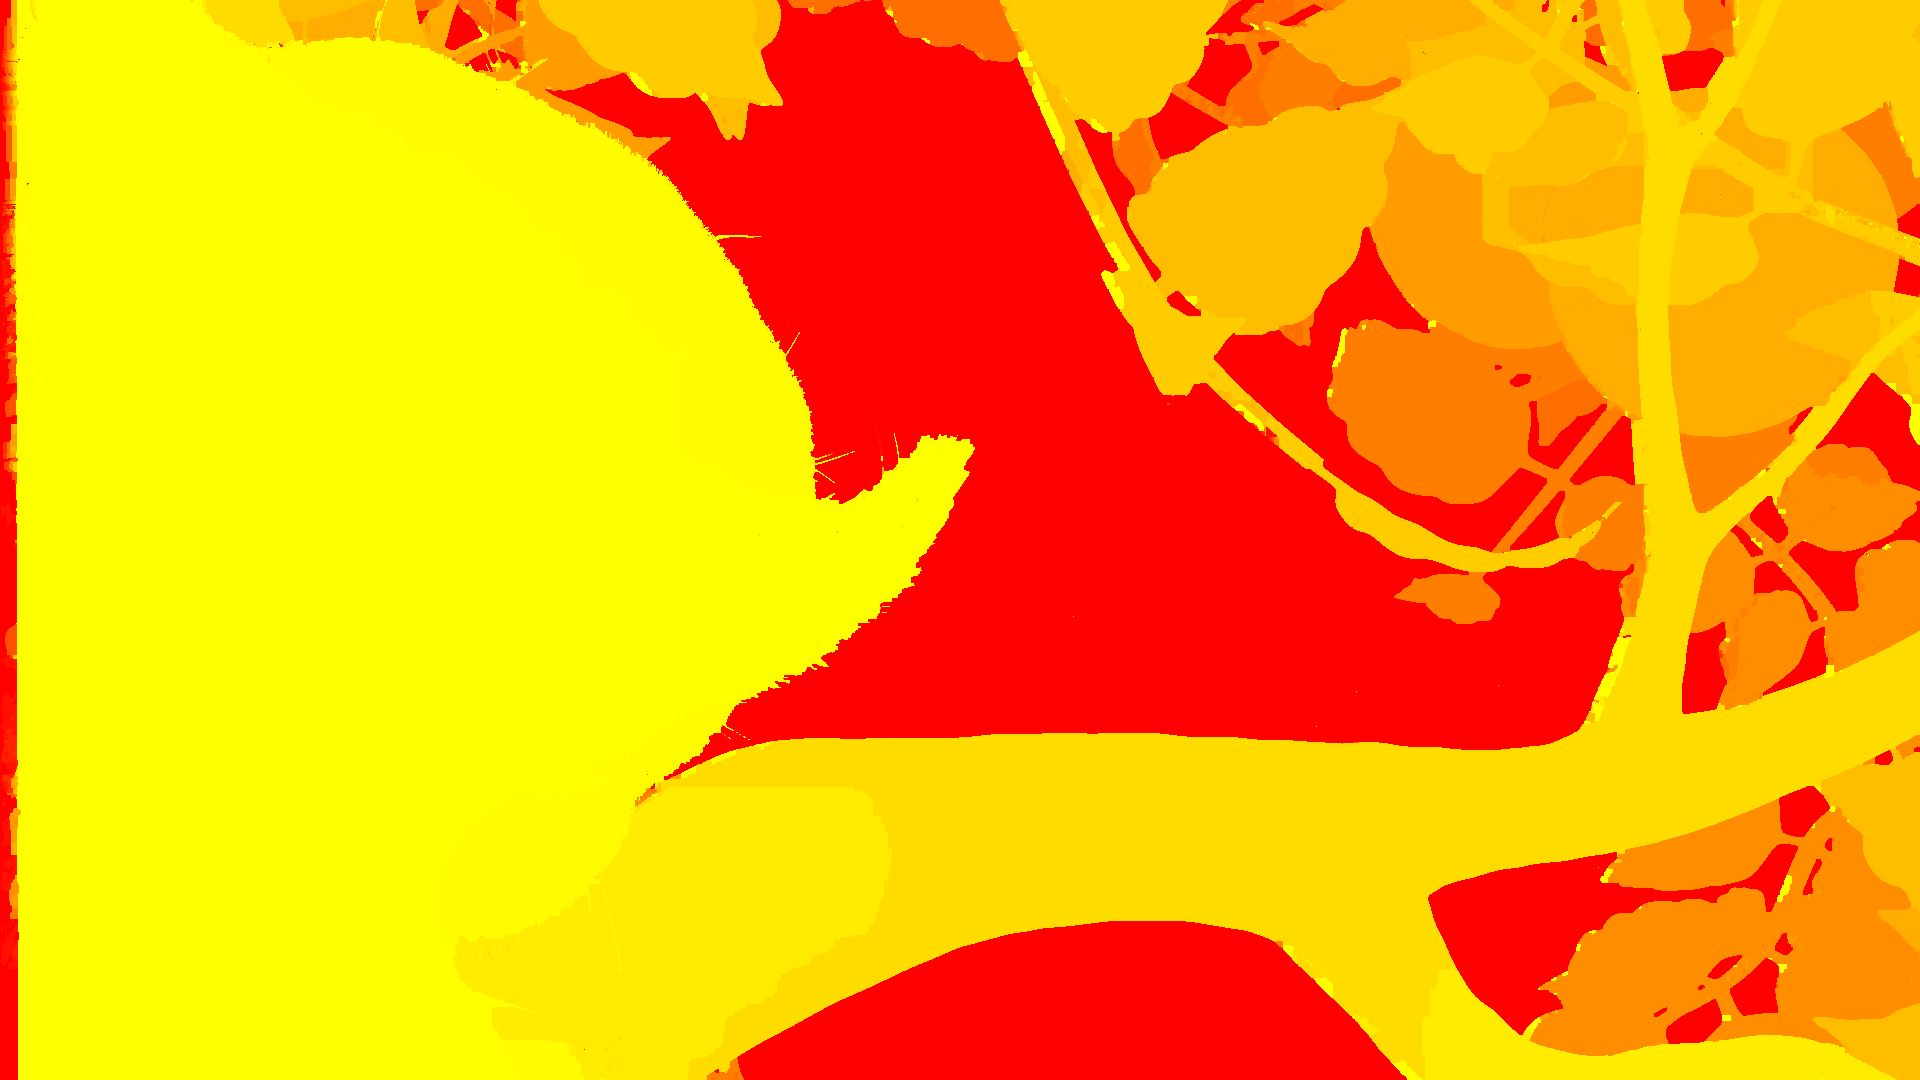
\includegraphics[width=0.47\textwidth]{src/images/svddd-03-heatmap-mrf.png}} &
\subfloat[ELAS output]{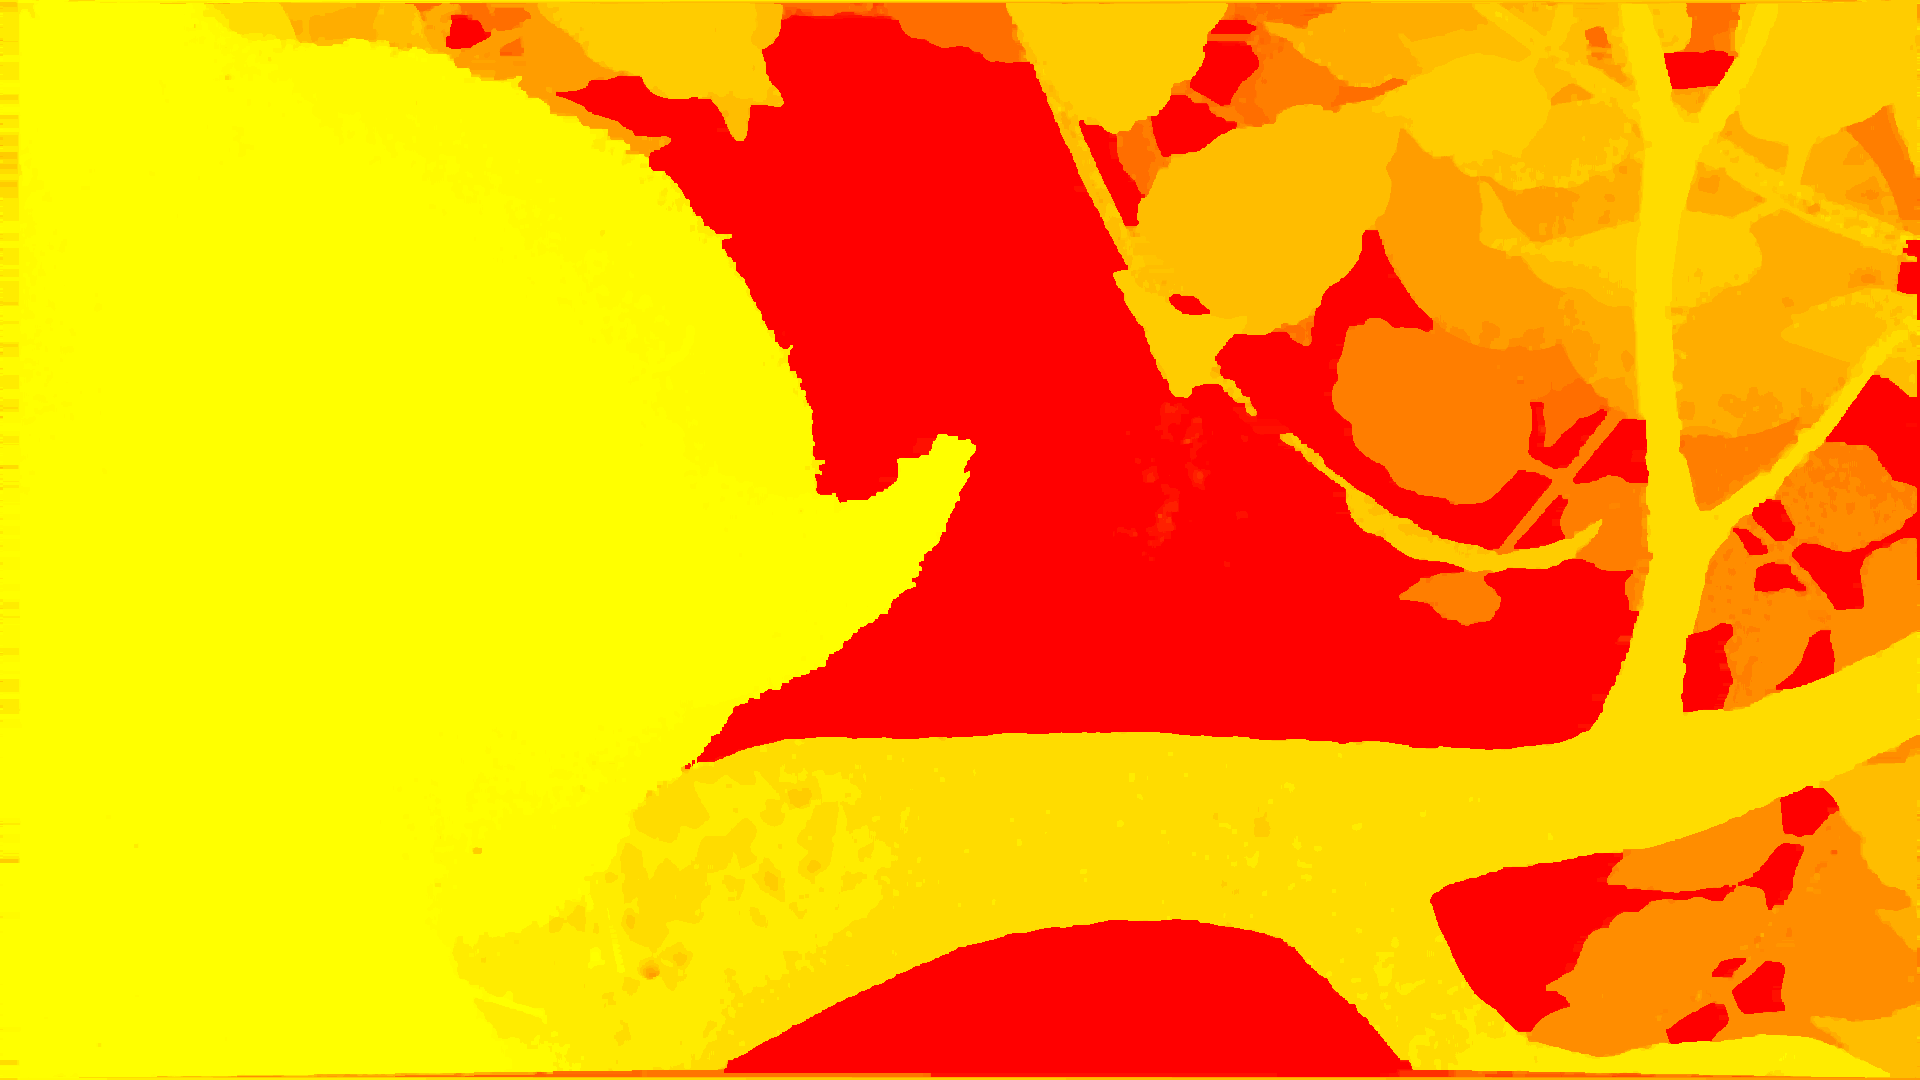
\includegraphics[width=0.47\textwidth]{src/images/svddd-03-heatmap-elas.png}} \\

\end{tabular}
\caption{Frame 01, scene 03 rabbit of the SVDDD dataset.}
\label{fig:svddd}
\end{figure}

\begin{figure}[h!]
  \centering
  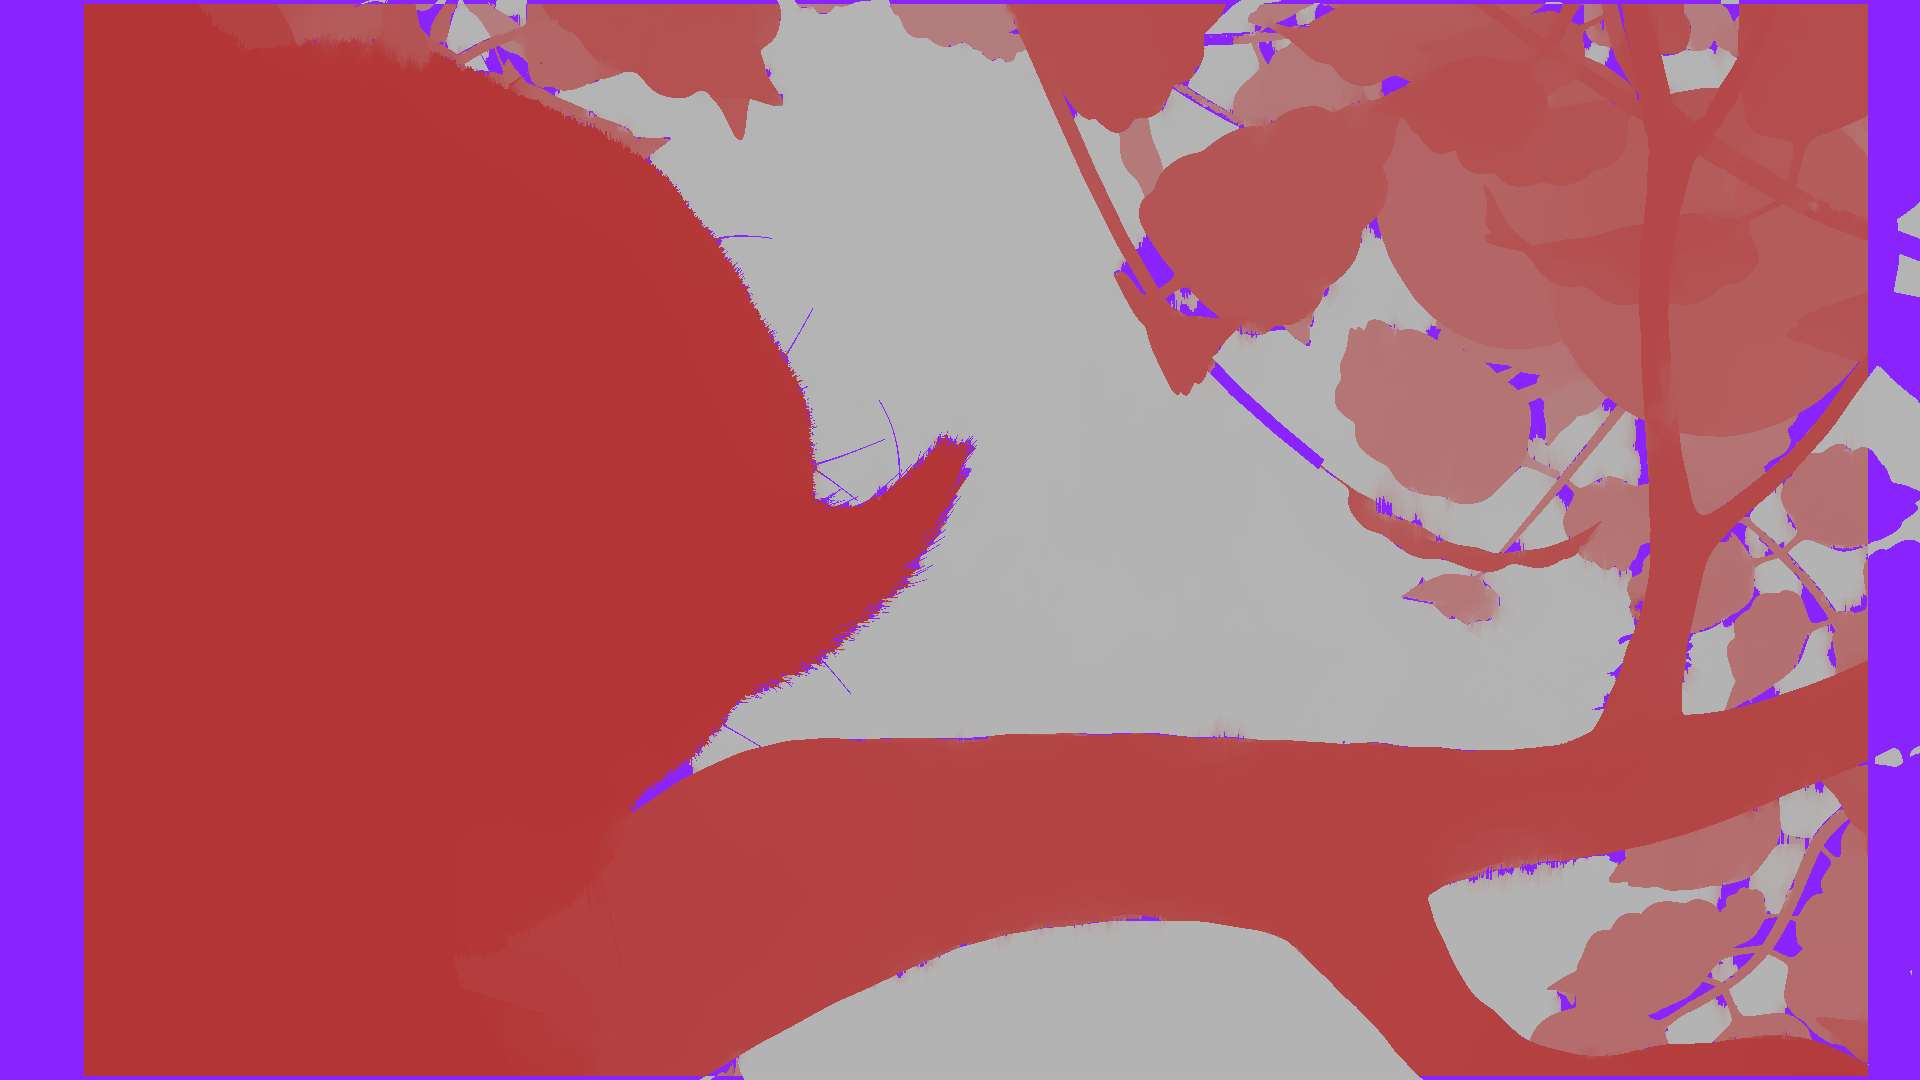
\includegraphics[width=1.0\textwidth]{src/images/svddd-03-heatmap-outliers.png}
  \caption{Heatmap of outliers with threshold of 4.0 pixels in computed disparity map with OpenCV SGBM, frame 01, scene 03 rabbit, SVDDD dataset.}
  \label{fig:svddd-07}
\end{figure}

\subsection{Smoothing over time}

\subsubsection{Result matrix}

Insert overview matrix.

\subsection{Runtime measurement}

Depict:

\begin{itemize}
  \item different performance of disparity algorithms,
  \item down-scaled performance,
  \item first down-scale, then run algorithms, then upscale, runtime,
  \item smoothing-over-time runtime.
\end{itemize}

\subsubsection{Result matrix}

\begin{landscape}
  \begin{table}[h!]
  \centering
  \begin{tabular}{cll|rrr}
    \hline
    \textbf{Rank} & \textbf{Method} & \textbf{Sequence} &  \textbf{Time} & \textbf{Time/MP} & \textbf{Quality index} \\ \hline \hline
    1 & StereoSGBM & SVDDD 02\_rabbit & 4.35\% & \cellcolor{green!60}5.43\% & 1.0 px \\
    2 & StereoBM & SVDDD 02\_rabbit & 4.35\% & 5.43\% & \cellcolor{red!60}1.1 px \\ \hline
  \end{tabular}
  \caption{Result matrix of runtime for videos}
  \label{tab:result-videos-runtime}
  \end{table}
\end{landscape}

\section{Discussion}

This is really important!


